\documentclass[12pt,a4paper,openright]{report}
\usepackage[italian]{babel}
\usepackage[utf8]{inputenc}
\usepackage{hyperref}
\usepackage{url}
%\usepackage{natbib}
\usepackage{graphicx}
\usepackage{makeidx}
\usepackage{listings}
\usepackage[square,numbers,sort]{natbib}
\usepackage{tabularx}
\usepackage{float}
\newcommand{\thesislang}{italian} % decommentare in caso di tesi in italiano
%\newcommand{\thesislang}{english} % commentare in caso di tesi in italiano
\usepackage{thesis-style}

% version
\newcommand{\versionmajor}{0}
\newcommand{\versionminor}{1}
\newcommand{\versionpatch}{2}
\newcommand{\version}{\versionmajor.\versionminor.\versionpatch}
\typeout{Document version: \version}

\title{\LARGE
    BDOnto: una Ontologia nel contesto dei Big Data e la Data Science  \\ \small Web Semantico
}

\author{
    Penazzi Paolo \\ \small paolo.penazzi@studio.unibo.it
    \and
    Parrinello Angelo \\ \small angelo.parrinello@studio.unibo.it
}

\date{\small Anno Accademico 2022-2023}
\makeindex

\begin{document}
\maketitle

\tableofcontents

\chapter{Introduzione}

Nel mondo contemporaneo, l'analisi dei dati ha assunto un ruolo centrale in una vasta gamma di settori, dalla ricerca scientifica all'industria e all'amministrazione pubblica. L'evoluzione rapida delle tecnologie e la crescente quantità di dati generati quotidianamente hanno portato alla necessità di modellare e rappresentare in modo accurato il vasto panorama di concetti, tecnologie e processi legati all'analisi dei dati e alla scienza dei dati. Questa necessità è stata quindi trasformata in una opportunità di progetto da \cite{BDOnto}.\\

Questa ontologia offre una rappresentazione semantica dettagliata e strutturata di diversi aspetti chiave di un settore in continua crescita. La progettazione dell'ontologia mira a coprire una vasta gamma di entità e concetti, tra cui le diverse fasi del processo di Data Science, le tecnologie impiegate, gli strumenti, i servizi, i linguaggi di programmazione e altro ancora. Il nostro obiettivo è sviluppare un'ontologia interessante e logica, basata sulla nostra esperienza e ispirata da riferimenti come \cite{BDOnto} e \cite{BDOnto_PhD}. Il progetto mira a esplorare gli aspetti chiave del Web Semantico, cercando di ottenere una comprensione più approfondita attraverso l'analisi di tali elementi.
\chapter{Studio del dominio}
In questa sezione svolgeremo un'analisi approfondita e dettagliata dei concetti, delle relazioni e delle caratteristiche rilevanti nel campo delle tecnologie legate ai Big Data e al processo di Data Science. Questo studio del dominio ha lo scopo di comprendere i vari aspetti che compongono il contesto dell'ontologia, inclusi i diversi passaggi del processo di Data Science, le tecnologie coinvolte, i linguaggi di programmazione, i servizi, gli strumenti e altri concetti pertinenti. Durante questo studio, abbiamo esaminato diverse fonti di partenza, analizzato documentazione tecnica e identificare le principali entità e relazioni che caratterizzano il dominio in oggetto. Questa fase è cruciale per una progettazione accurata dell'ontologia, consentendo di modellare in modo efficace la complessità e la diversità del dominio preso in considerazione.

\section{Problema e Motivazione}\label{sec:motivazione}
Il numero di realtà che si occupano di prodotti in ambito Big Data è salita. Un censimento del 2021 \cite{bigdatalandscape2021} sulle tecnologie legate al mondo del Machine Learning, AI e Big Data ha mostrato come sono più di 2000 prodotti legati a questo ambito ed i numero, così come i trend, stanno cambiando rapidamente. Non sorprende quindi che la domanda di esperti in tale ambito è in aumento. Di conseguenza, l'aumento della complessità e della cardinalità dei sistemi legati al mondo dei Big Data porta inevitabilmente con sè un costante aumento di indecisione e momenti di stallo, ogni qualvolta che un team deve decidere quale tecnologia adottare o che step seguire all'interno di un processo inerente alla Data Science.\\ 

L'espansione delle opzioni disponibili per soddisfare specifiche esigenze non è necessariamente negativa, ma può portare all'aumento dei costi, ad esempio, nelle ore uomo impiegate nella scelta degli strumenti per l'analisi dei dati. Attualmente, l'unica classificazione che cerca di offrire una visione d'insieme in questo contesto è rappresentata da \cite{BDOnto}. Tuttavia, questa soluzione non è open source, rendendola non direttamente utilizzabile. La mancanza di standardizzazione in diverse aree nei settori della Data Science e del Big Data è ciò che ha attirato la nostra attenzione su questo problema.

\section{Analisi del dominio}\label{sec:analisi_dominio}
Il progetto è incentrato su due domini: quello della Data Science e delle tecnologie Big Data. Il contesto del nostro studio è per sua natura molto variegato e complesso, quindi si presta bene ad un tentativo di standardizzazione. Inoltre, grazie alla sua dualità questo può essere facilmente esteso e applicabile a numerosi progetti.\\

Il processo di definizione dei requisiti nasce dallo studio di \cite{BDOnto} e \cite{BDOnto_PhD}. Partendo dall'analisi proposta in particolare in \cite{BDOnto}, sono state fin da subito individuate le seguenti definizioni:
\begin{table}[H] 
\centering 
\begin{tabular}{cp{40ex}} 
\hline {\textbf{Termine}}& \multicolumn{1}{c}{\textbf{Definizione}}\\ 
\hline Big Data Technology &  Strumenti, hardware e servizi progettati per gestire ed elaborare set di dati enormi e complessi, consentendo alle organizzazioni di archiviare, analizzare ed estrarre informazioni preziose da grandi quantità di dati.\\ 
\hline Data Science Process & Approccio sistematico e iterativo per risolvere problemi complessi raccogliendo, pulendo, analizzando e interpretando i dati per ricavare informazioni preziose e prendere decisioni informate.\\ 
\hline 
\end{tabular}
\end{table}
\newpage
Focalizzandosi sul concetto di \textbf{Data Science Process} e seguendo gli step proposti in \cite{BDOnto}, siamo giunti alla conclusione che i passi principali di questo processo si potevano riassumere in:
\begin{table}[H] 
\centering 
\begin{tabular}{cp{40ex}} 
\hline {\textbf{Termine}}& \multicolumn{1}{c}{\textbf{Definizione}}\\ 
\hline Data Provision &  Collegamento e integrazione delle fonti di dati, memorizzazione dei dati grezzi.\\ 
\hline Data Preparation & Pulizia, trasformazione e modellazione della struttura dei dati.\\ 
\hline Data Analysis & Riconoscimento, modellazione ed estrazione di informazioni dai dati.\\ 
\hline Data Visualization & Presentazione visiva o implementazione dei risultati.\\ 
\hline 
\end{tabular}
\end{table}

\section{Riuso di ontologie esistenti}
Ad inizio opera, sono state valutate diverse opzioni ed ontologie da cui partire. \\

Prime fra tutte la Software Ontology (SWO) \cite{SWO}, la Information Artifact Ontology (IAO) \cite{IAO} e la Ontology of Data Mining (Onto-DM) \cite{OntoDM} che sono state analizzate anche nel paper di riferimento. Onto-DM descrive diverse fasi dei processi di data mining, tipi di dati e loro elaborazione. La SWO descrive strumenti e algoritmi utilizzati nella bioinformatica. La IAO si concentra più su oggetti generali al fine di rappresentare una sorta di ontologia ponte. La OntoDM \cite{OntoDM}, è stata scartata fin da subito in quanto non rintracciabile attraverso le nostre ricerche online. Per quanto riguarda la IAO \cite{IAO} e la SWO \cite{SWO} si è deciso di non utilizzarle ma di cercare delle alternative: l'estensione e la eterogeneità di queste due ontologie sono i due motivi principali del suo non impiego. Volevamo porre maggior focus su i domini da noi ricercati e quindi si è valutato in un primo momento di non utilizzarle ed eventulamente in seguito di integrarle nel progetto. La tecnica che si sarebbe utilizzate sarebbe stata quella proposta in \cite{BDOnto} ovvero un'estrazione mirata su concetti già espressi da queste ontologie e riutilizzabili all'interno del nostro lavoro.\\

In seguito, sono state studiate tre ulteriori ontologie: la Code Ontology \cite{Code_Ontology}, la Data License Ontology (DLO) \cite{DLO} e la Hardware Ontology \cite{Hardware_Ontology}. La prima è un'ontologia pensata per modellare linguaggi di programmazione object-oriented e codice sorgente. La seconda è una mini-ontologia contenente le classi per ciascuna delle licenze da Open Data Commons. Mentre l'ultima è una ontologia estremamente ricca e verticale su tutto l'aspetto tecnologico hardware.\\

Valutando tutti i pro e contro di ogni ontologia proposta in questa sezione, è stato scelto di impiegare la DLO \cite{DLO} e la Hardware Ontology \cite{Hardware_Ontology} per rappresentare concetti estremamente importanti e direttamente legati al mondo Big Data quali l'hardware e la licenza. Va fatto notare che la Code Ontology \cite{Code_Ontology} è un'ontologia estremamente promettente, strutturata e documentata che fin da subito è stata integrata nel progetto. In seguito però si è notato come in realtà questa integrazione fosse fine a sè stessa, in quanto non venivano impiegate nessuna delle classi o proprietà al suo interno definite e per questo è stata eliminata dall'elaborato.
 
\section{Costruzione della Tassonomia}
La tassonomia inizia è stata sviluppata focalizzandosi sui concetti di Big Data Technology e Data Science Step. Di conseguenza si è modellata la gerarchia delle classi:
\begin{itemize}
    \item \textbf{License}, per modellare un autorizzazione legale su opere come il software (direttamente integrata da DLO \cite{DLO});
    \item \textbf{Hardware}, per modellare la componente fisica di un sistema informatico (direttamente integrata dalla Hardware Ontology \cite{Hardware_Ontology});
     \item \textbf{Big Data Technology}, per modellare una tecnologia legata al mondo dei Big Data;
     \item \textbf{Data Science Process}, per modellare una componente del processo di un progetto di Data Science.
\end{itemize}
Ogni classe principale è composta da una o più sottoclassi. Per brevità non verranno elencate tutte ma spiegheremo solamente quelle principali:
\begin{itemize}
    \item All'interno della classe \textbf{Big Data Technology} troviamo la classi \textbf{Big Data Service}, che modella i principali servizi utilizzati nei progetti Big Data, e \textbf{Big Data Tool}, che cerca di racchiudere tutti i tool/software pensati per grandi quantità di dati ed i \textbf{Programming Language}, che modella un linguaggio di programmazione;
    \item Come sottoclasse di \textbf{Data Science Process}, troviamo i già citati step che la compongono (\textbf{General Steps}) e soprattutto le operazioni, \textbf{Operation}, che possono far parte del ciclo di vita di un progetto di Data Science (i.e. \textbf{Data Processing} o \textbf{Classification}).
    \item Infine, come estensione della ontologia importata Ontology Hardware \cite{Hardware_Ontology} troviamo la classe \textbf{Server} (ovvero Commodity Server), ovvero un concetto legato alle macchine fisiche impiegate per elaborare grandi quantità di dati. Una naturale estensione di tale classe è \textbf{Server Enterprise} ovvero dei server con caratteristiche migliori rispetto al caso base.
\end{itemize}

Le classi principali, così come le sottoclassi, sono disgiunte tra loro in quanto ritenuto concettualmente non possibile l'appartenenza di un'istanza a più classi diverse. Alcune di queste classi presentano delle \textit{equivalenze}: sarà poi il \textbf{Reasoner} a classificare le istanze.\\

In seguito (Figura \ref*{fig:classi_bdonto}) si può vedere la struttura dell'ontologia, con le classi e sottoclassi principali.

\begin{figure}[H]
    \centering
    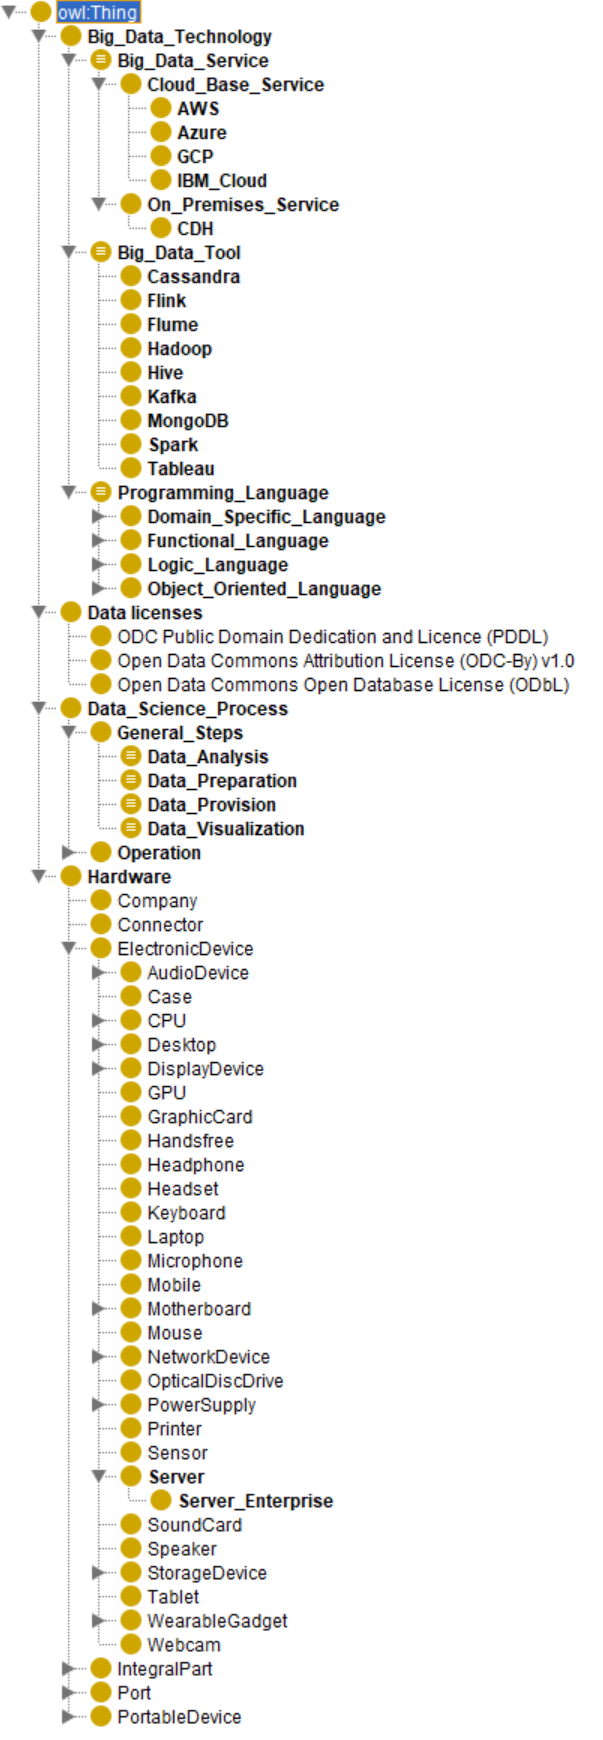
\includegraphics[height=12.5cm]{docs/images/taxonomyWS.PNG}
    \caption{Struttura dell'ontologia BDOnto.}
    \label{fig:classi_bdonto}
\end{figure}
Tutte le classi sono state determinate seguendo un approccio iterativo, cambiando più volte la struttura generale a seconda delle esigenze che nel corso dello svluppo nascevano e secondo ciò che veniva definito all'interno della letteratura.\\

Per facilitare il lettore nella comprensione, ecco un estratto (Figura \ref{fig:owlviz_bdonto}) della gerarchia delle classi creata tramite il plugin \textbf{OWLViz} presente in \textbf{Protégé}.

\begin{figure}[H]
    \centering
    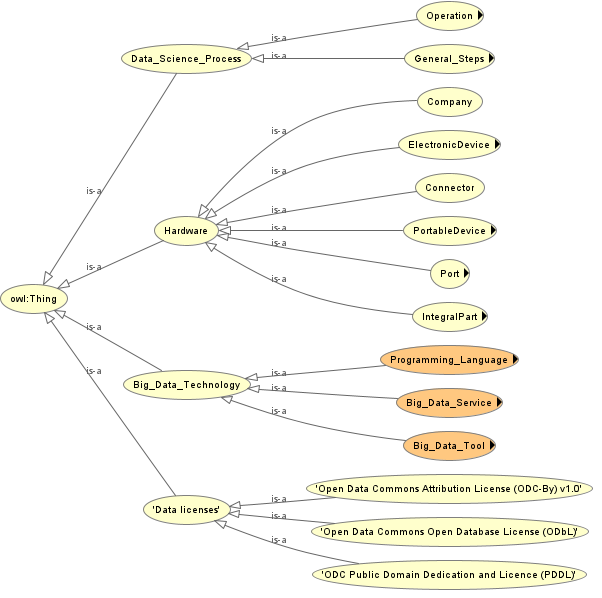
\includegraphics[width=15cm]{docs/images/owlvizBdonto.png}
    \caption{Struttura dell'ontologia BDOnto attraverso \textit{OWLViz}.}
    \label{fig:owlviz_bdonto}
\end{figure}
\newpage
\section{Valutazione delle Object Properties}
Le object properties hanno aiutano a modellare le relazioni e le interconnessioni tra le diverse entità nel dominio, consentendo poi al reasoner di inferire nuove informazioni sulla base di tali relazioni. Inoltre, agevolano la ricerca e l'interrogazione dell'ontologia, consentendo agli utenti di recuperare informazioni specifiche attraverso le connessioni definite. L'analisi del dominio ha permesso, in seguito, di individuare quelle proprietà specifiche che modellano i vincoli tra classi negli individui.\\

Nella figura seguente (Figura \ref*{fig:proprieta_bdonto}) si notano molte proprietà, tante delle quali sono state importate dalle ontologie estese sopra nominate.
\begin{figure}[H]
    \centering
    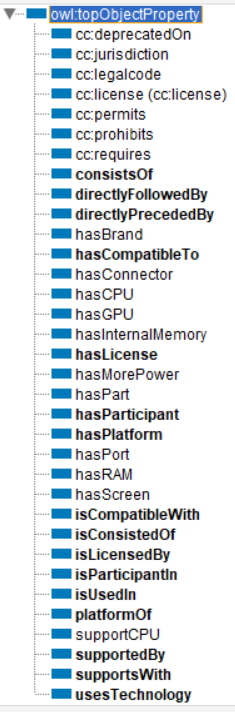
\includegraphics[width=4.2cm]{docs/images/datapropWS.PNG}
    \caption{Object properties dell'ontologia BDOnto. In grassetto le proprietà definite da noi.}
    \label{fig:proprieta_bdonto}
\end{figure}

Per quanto riguarda l'ontologia progettata, ogni proprietà presenta la sua inversa, il che è una buona pratica per consentire la navigazione bidirezionale nell'ontologia.\\

Sono quindi state modellate le seguenti proprietà:
\begin{itemize}
    \item \textbf{consistsOf}: modella le operazioni che possono fare parte di uno specifico step del Data Science Process;
    \item \textbf{isConsistedOf}: proprietà inversa di \textit{consistsOf};
    \item \textbf{directlyFollowedBy}: proprietà \textit{funzionale ed inversa funzionale} che modella l'ordine degli step in un progetto di Data Science;
    \item \textbf{directlyPrecededBy}: proprietà \textit{funzionale ed inversa funzionale} di \textit{directlyFollowedBy};
    \item \textbf{isCompatibleWith}: proprietà \textit{transitiva}, che modella la compatibilità tra due sistemi;
    \item \textbf{hasCompatibleTo}: proprietà \textit{transitivia} ed inversa di \textit{isCompatibleWith};
    \item \textbf{hasLicense}: proprietà \textit{funzionale inversa} che modella la relazione di regolamentazione legale da parte di una licenza su un tool;
    \item \textbf{isLicensedBy}: proprietà inversa di \textit{hasLicense};
    \item \textbf{hasParticipant}: modella la partecipazione di un elemento all'interno di un dato step della Data Science;
    \item \textbf{isParticipantIn}: proprietà inversa di \textit{hasParticipant};
    \item \textbf{supportsWith}: modella il supporto di una certa tecnologia o linguaggio o altro ancora da parte di un dato tool o tecnologia;
    \item \textbf{supportedBy}: proprietà inversa di \textit{supportsWith};
    \item \textbf{usesTechnology}: modella la relazione di impiego di una tecnologia da parte di un'altra tecnologia;
    \item \textbf{isUsedIn}: proprietà inversa di \textit{usesTechnology};
    \item \textbf{hasPlatform}: proprietà \textit{funzionale} modella la compagnia che regola, sviluppa, detiene una tecnologia;
    \item \textbf{platformOf}: proprietà inversa di \textit{hasPlatform}.
\end{itemize}

Qualora ritenevamo avesse senso modellare il concetto di \textit{Dominio} e \textit{Range} all'interno di queste proprietà è stato fatto (in modo tale da facilitare il reasoner), altrimenti è stata lasciata piena libertà di utilizzo (ed evitare 'inaspettate' classificazioni, come suggerito in \cite{Protege_Tutorial}).

\section{Valutazioni delle Data Properties}

Durante l'analisi iniziale, le varie entità presenti non risultavano caratterizzate da valori numerici, quindi non si presentavano \textit{Data Properties}. Questa caratteristica, che rendeva il dominio poco interessante e molto "tassonomico", andava superata. Ci siamo quindi sforzati nel cercare informazioni numeriche per le entità di questo dominio. Dopo diversi tentativi, sono state modellate delle proprietà numeriche per le principali classi della tassonomia, che hanno particolarmente arricchito il progetto. Queste proprietà sono state fondamentali in fase di modellazione di alcune classi di equivalenza. Un esempio, è la classe Big Data Tool è equivalente ad una Big Data Technology che supporta almeno un linguaggio di programmazione, che ha una certa dimensione in MB, ha una certa versione, ecc.\\

Nello specifico sono state modellate le seguenti Data Properties:
\begin{itemize}
    \item \textbf{hasAverageCost}: indica il costo medio (in dollari) di una tecnologia; deve avere un valore maggiore o uguale a 0.0.
    \item \textbf{hasAverageSize}: indica la dimensione media del software (in MB); deve avere un valore maggiore o uguale a 0.0.
    \item \textbf{hasDifficultyLevel}: indica la difficoltà nell'usare una tecnologia; i valori variano da 1 (facile) a 5 (estremamente difficile).
    \item \textbf{hasEndOfSupportDate}: indica la data nella quale una tecnologia smetterà di essere supportata o ha cessato di essere supportata.
    \item \textbf{hasFullName}: indica il nome completo di quella entità.
    \item \textbf{hasLearningCurve}: indica la pendenza della curva di apprendimento di una data tecnologia; i valori variano da 1 (ritmo rapido) a 5 (ritmo estremamente lento).
    \item \textbf{hasStartingDate}: indica la data nella quale l'entità è nata.
    \item \textbf{hasVersion}: indica la versione della tecnologia.
    \item \textbf{hasParadigm}: indica il paradigma di programmazione supportato dal linguaggio (es. imperativo, dichiarativo, orientato agli oggetti).
    \item \textbf{hasLifespan}: indica la durata (in mesi) del supporto a tale tecnologia.
\end{itemize}

Abbiamo modellato i concetti di \textit{Dominio} e \textit{Range} all'interno di queste proprietà solo quando lo abbiamo ritenuto opportuno, seguendo un approccio flessibile.\\

Le ontologie importate portavano con sè un numero considerevole di proprietà quindi qui di seguito vengono mostrate solo alcune delle Data Properties presenti all'interno dell'ontologia:

\begin{figure}[H]
    \centering
    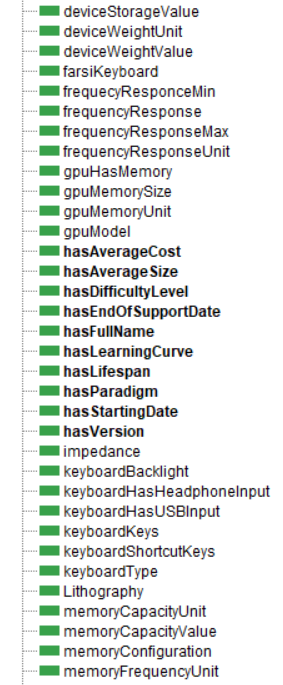
\includegraphics[height=14cm]{docs/images/objpropWS.PNG}
    \caption{Data properties dell'ontologia. In grassetto le proprietà definite da noi.}
    \label{fig:datap_bdonto}
\end{figure}


\chapter{Modellazione e sviluppo dell'ontologia}
Durante lo sviluppo dell'ontologia si è cercato il più possibile di integrare le ontologie già esistenti citate, in modo da non dover ripetere la modellazione di classi e proprietà già definite e rendere tutto più consistente.\\

Tutte le classi che classi che presentano una equivalenza sono state definite come \textbf{Defined Class} ovvero una classe che ha almeno una condizione necessaria e sufficente (all'interno di Protègè queste classi vengono chiamate Equivalent Class). Nella pratica stiamo dicendo che se un individuo è un membro della classe A deve soddisfare le condizioni ed inoltre possiamo dire che se un individuo soddisfa queste condizioni allora deve essere un membro della classe A. Questa scelta è stata fatta per aiutare il reasoner a inferire meglio le classi (si veda \cite{definedclass}).

\section{Big Data Technology}
La classe \textbf{Big Data Technololgy} è l'entità principale dell'ontologia, la quale è una generificazione delle tre sottoclassi \textbf{Big Data Service}, \textbf{Big Data Tool} e \textbf{Programming Language}. L'importanza di questa classe risiede nel fatto che ogni specializzazione di essa deriva da essa stessa e quindi ognuna delle sottoclassi presenterà una equivalenza diretta alla classe madre.\\

Alcune delle proprietà (numeriche e non) sono applicabili a tutte le entità di tipo Big Data Technology. Alcune di queste però, sono necessarie affinchè una tecnologia si specializzi in una sottoclasse. Nelle sezioni seguenti anallizzeremo più approfonditamente alcune delle classi più importanti dell'ontologia.
\newpage
\subsection{Big Data Tool}
Una software specifico per i Big Data è definito \textbf{Big Data Tool}. Attualmente sono stati modellati solo alcuni tra i molteplici tool Big Data, come si evince dalla figura \ref{fig:bdtool_graph}.

\begin{figure}[H]
    \centering
    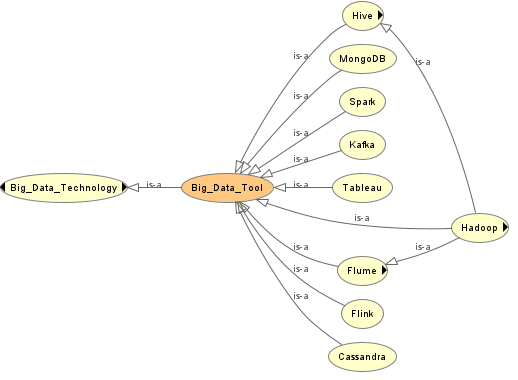
\includegraphics[width=12cm]{docs/images/bdtoolowlviz.png}
    \caption{Gerarchia dei Big Data Tool creato su Protègè tramite il plugin OWLViz.}
    \label{fig:bdtool_graph}
\end{figure}

Una tecnologia Big Data per essere definita Tool dovrà rispettare alcune condizioni necessarie e sufficienti. Per ogni Tool sono presenti:
\begin{verbatim}
Big_Data_Technology
    and (supportsWith some Programming_Language)
    and (hasAverageSize exactly 1 xsd:float)
    and (hasDifficultyLevel exactly 1 xsd:int)
    and (hasEndOfSupportDate exactly 1 xsd:dateTime)
    and (hasLearningCurve exactly 1 xsd:int)
    and (hasVersion exactly 1 xsd:string)
\end{verbatim}

\newpage

Come si può vedere nell'esempio di istanza in figura \ref{fig:cassandra_graph} tutte le condizioni affinchè una tecnologia venga classificata come tool sono state soddisfatte ed è inoltre presente un'altra istanza (\textit{Cassandra\_V.2.7.9}) che presenta una retrocompatibilità con l'istanza in questione: questa informazione è resa possibile dal reasoner e dalla proprietà inversa \textit{isCompatibleWith}.

\begin{figure}[H]
    \centering
    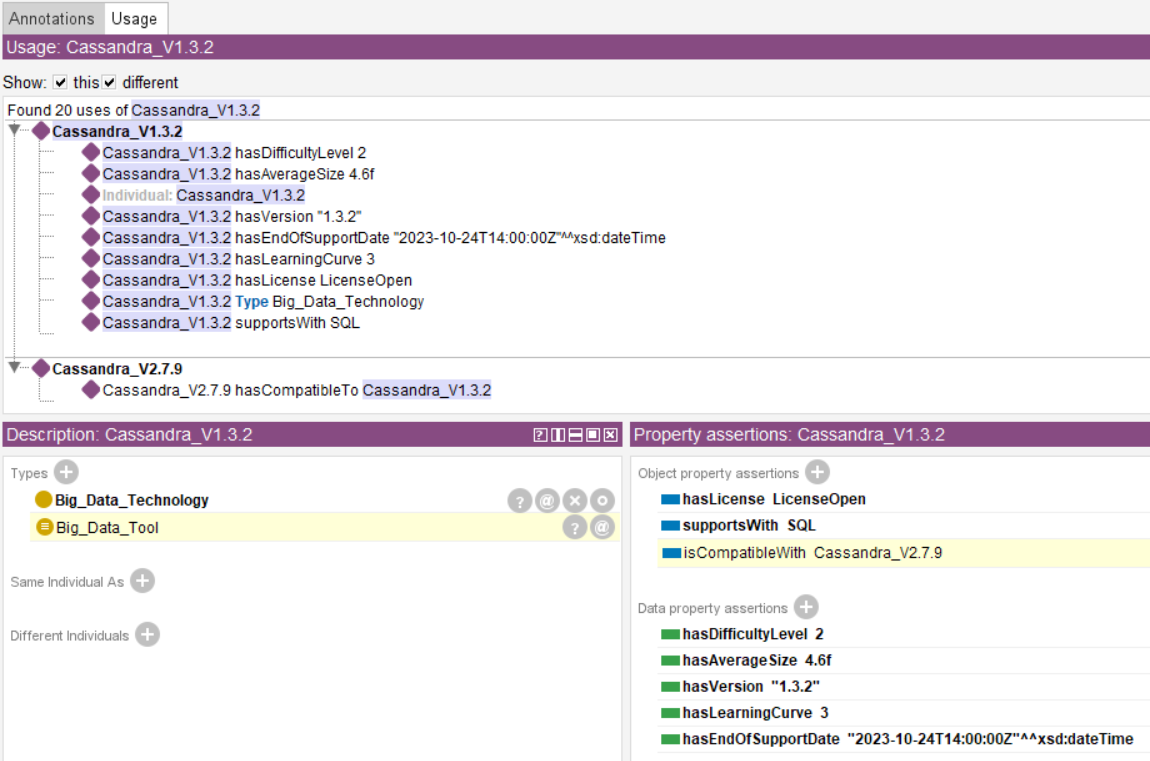
\includegraphics[width=15cm]{docs/images/cassandraex.PNG}
    \caption{Esempio di istanza di Big Data Technology classificata come Big Data Tool dal reasoner di Protègè, Pellet.}
    \label{fig:cassandra_graph}
\end{figure}

Infine, è stato modellato anche il concetto di impiego di un tool da parte di un altro. L'esempio migliore che si possa fare è Hadoop che consiste di tante tecnologie (es. Flume). Questa peculiarità è modellata con l'object property chiamata \textit{usesTechnology}.
\newpage
\subsection{Big Data Service}
Un servizio Big Data è un'offerta o una piattaforma fornita da un fornitore di servizi che consente alle organizzazioni di gestire, analizzare e sfruttare grandi volumi di dati in modo efficiente e scalabile. Tipicamente questi servizi offrono delle soluzioni che consentono l'utilizzo di software all'interno dei lori sistemi. Come si vede dalla figura \ref{fig:bdservice_graph}, l'ontologia prevede due tipi di soluzioni: quella cloud e quella on-premises.

\begin{figure}[H]
    \centering
    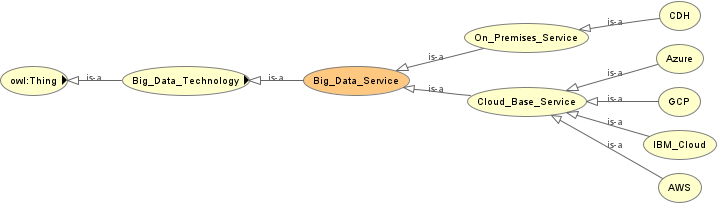
\includegraphics[width=12cm]{docs/images/bdserviceowlviz.png}
    \caption{Gerarchia dei Big Data Service creato su Protègè tramite il plugin OWLViz.}
    \label{fig:bdservice_graph}
\end{figure}

Come per i tool, anche i servizi sono un'estensione delle tecnologie big data e quindi presentano una condizione necessaria e sufficente:
\begin{verbatim}
Big_Data_Technology
 and (supportsWith some Big_Data_Tool)
 and (hasPlatform some Company)
 and (hasAverageCost exactly 1 xsd:float)
 and (hasDifficultyLevel exactly 1 xsd:int)
 and (hasLearningCurve exactly 1 xsd:int)
 and (hasVersion exactly 1 xsd:string)
\end{verbatim}

Il fornitore che offre un servizio o che dà la possibilità di installare il proprio servizio in locale è una proprietà fondamentale dei servizi Big Data, come si evince dalla figure \ref{fig:awsex_graph}.

\begin{figure}[H]
    \centering
    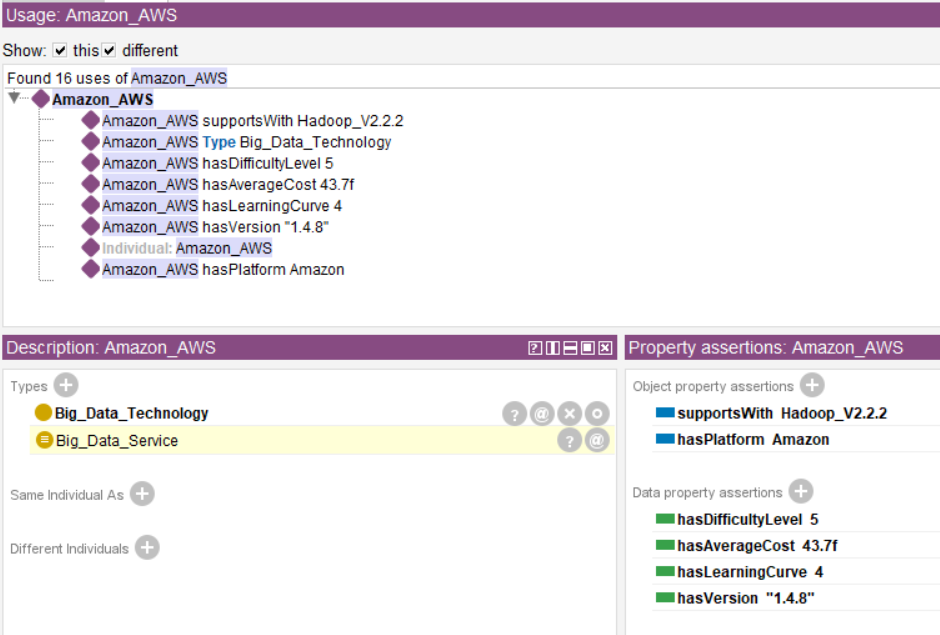
\includegraphics[width=15cm]{docs/images/awsex.PNG}
    \caption{Esempio di istanza di Big Data Technology classificata come Big Data Service dal reasoner di Protègè, Pellet.}
    \label{fig:awsex_graph}
\end{figure}

\section{Data Science Process}
Il Data Science Process è una sequenza organizzata di attività che mira a estrarre valore e conoscenza dai dati: questa classe rappresenta la macro-attività di questo processo.\\

In generale, questo processo può variare leggermente a seconda del contesto e degli obiettivi specifici, ma in questo progetto ci basiamo sulla definizione data in \cite{naous2017analytics} e \cite{BDOnto}. La sequenza di azioni svolte durante un progetto legato al mondo della Data Science, comprende degli step predefiniti (es. Data Analysis) che a loro volta comprendono delle operazioni che vengono svolte. Le operazioni che vengono svolte tendono ad essere mappate ad uno step della sequenza. Ad esempio, l'operazione di Data Gathering viene svolta nello step di Data Provision. Partendo quindi dalla classe madre, Data Science Process, troviamo due sottoclassi principali, General Steps e Operation, come si evince dalla figura \ref{fig:dataproc}.
\begin{figure}[H]
    \centering
    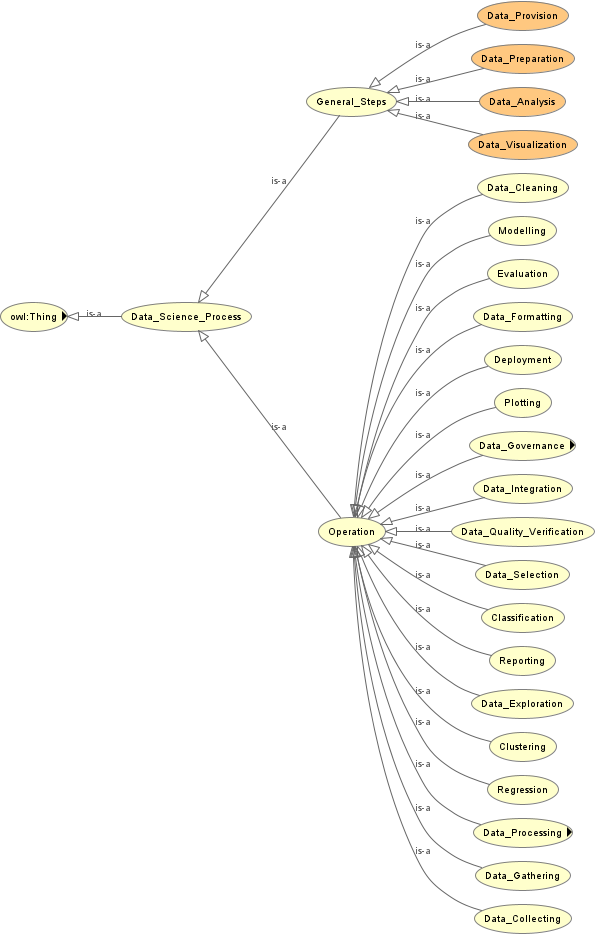
\includegraphics[height=13cm]{docs/images/dataprocowlviz.png}
    \caption{Gerarchia del Data Science Process, con una vista sulla due sottoclassi principali: General Steps e Operation}
    \label{fig:dataproc}
\end{figure}
\subsection{General Steps}
Per descrivere le operazioni di un Data Science Process, è stata creata la classe General Steps. Il flow, e quindi l'ordine, di queste operazioni è caratterizzato dalla proprietà \textit{directlyFollowedBy} che, come si può facilmente intuire, regola lo step successivo ad uno dato. Troviamo quattro step, Data Provision, Data Preparation, Data Analysis e Data Visualization,il cui ordine è mostrato in figura \ref{fig:hasSubclass}, che presenta anche una legenda del grafo.
\begin{figure}[H]
    \centering
    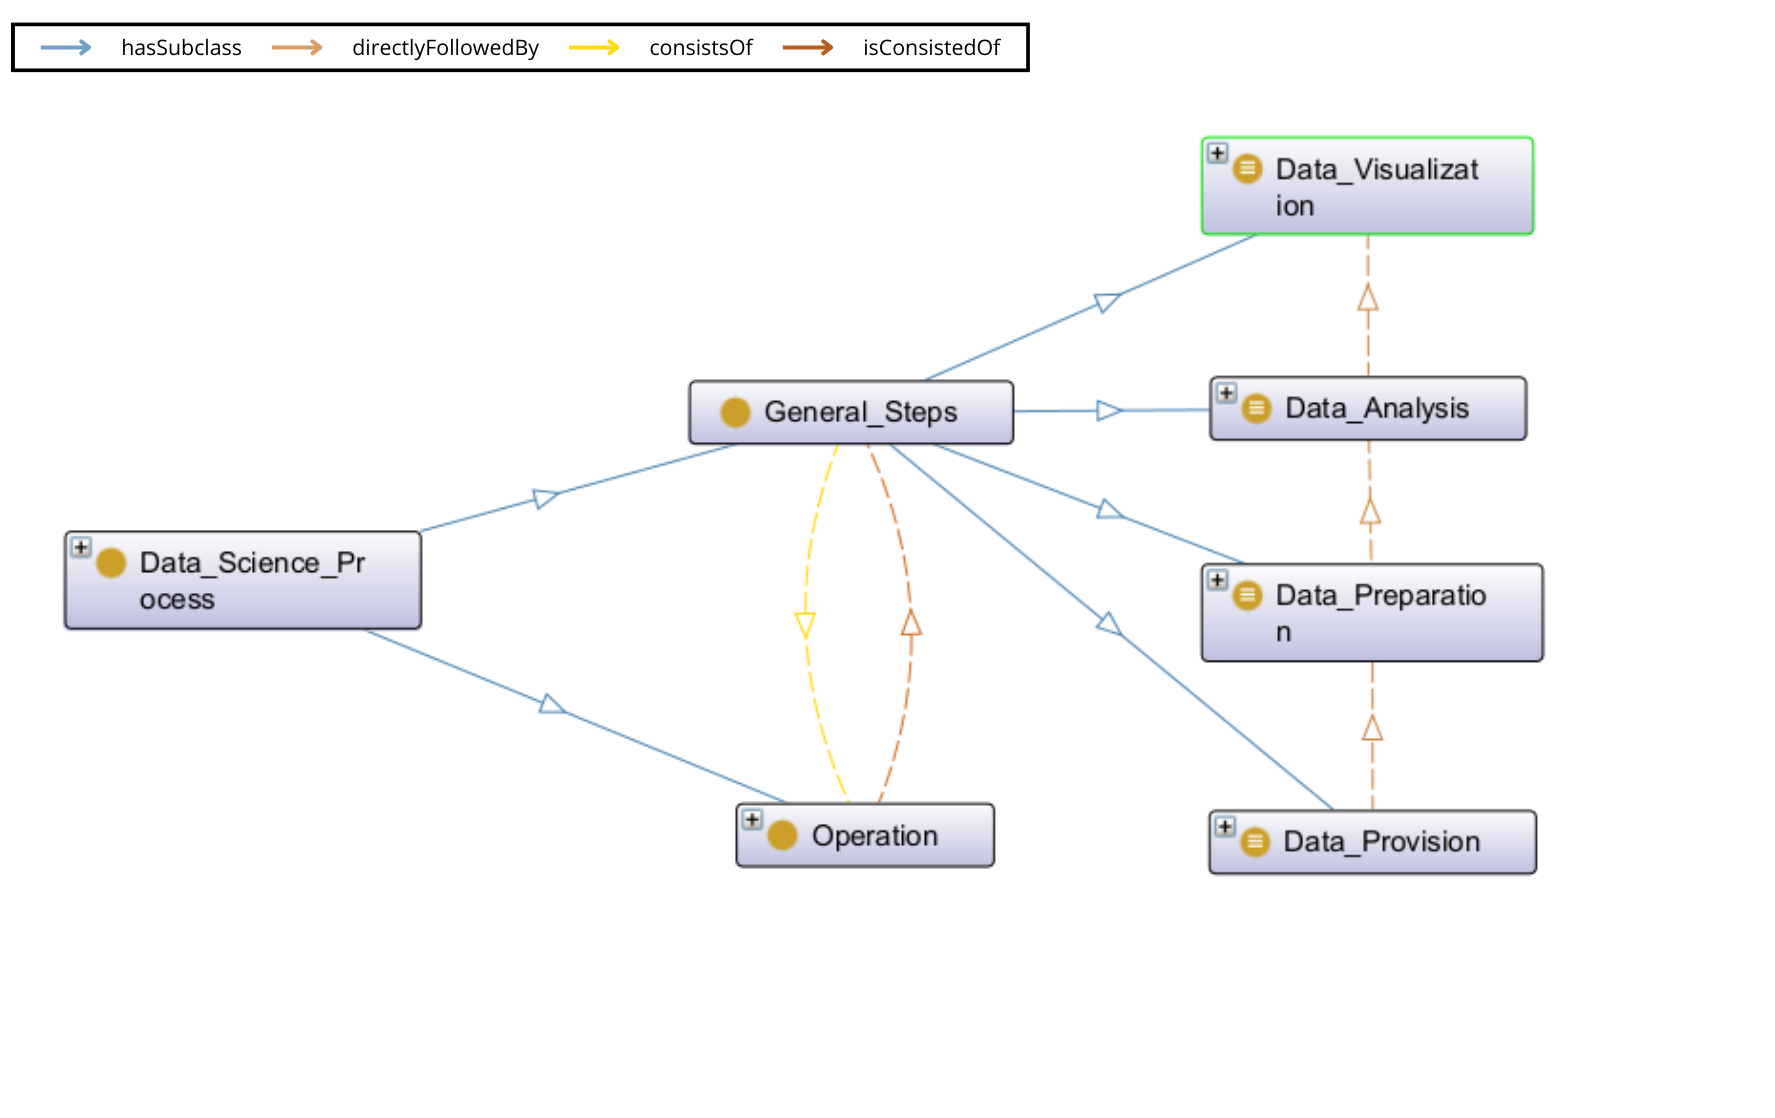
\includegraphics[width=12cm]{docs/images/hasSubclass.png}
    \caption{Ordinamento degli step all'interno di un processo di Data Science, rappresentato graficamente dal plugin OntoGraf all'interno di Protègè.}
    \label{fig:hasSubclass}
\end{figure}

Ogni specifico step è sottoclasse di General Steps, con obiettivi e rappresentazioni diversi. Ad esempio, la fase di Data Analysis punta a esaminare ed interpretare i dati mentre quella di Data Visualization si occuperà per lo più della interpretabilità dei dati. È intuibile quindi che ogni fase avrà operazioni diverse: questa relazione è modellata dalla proprietà \textit{consistsOf} (e dalla sua inversa \textit{isConsistedOf}). Si prenda come esempio la classe \textit{Data Analysis} e la sua descrizione mostrata in figura \ref{fig:data_anal}.
\begin{figure}[H]
    \centering
    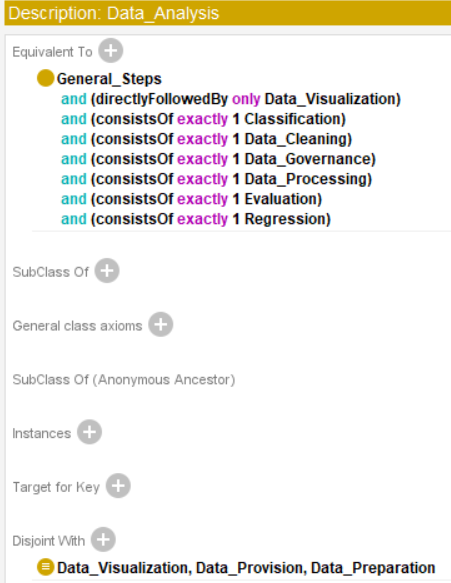
\includegraphics[height=6.3cm]{docs/images/datanaldesc.PNG}
    \caption{Descrizione della classe Data Analysis.}
    \label{fig:data_anal}
\end{figure}

Siccome ogni specifico step può essere visto come uno step generico che comprende determinate operazioni, è stato deciso di modellare questa peculiarità all'interno di una equivalenza per ognuno dei singoli step. Prendiamo il caso della classe \textit{Data Preparation}:

\begin{verbatim}
General_Steps
 and (directlyFollowedBy only Data_Analysis)
 and (consistsOf exactly 1 Clustering)
 and (consistsOf exactly 1 Data_Exploration)
 and (consistsOf exactly 1 Data_Formatting)
 and (consistsOf exactly 1 Data_Governance)
 and (consistsOf exactly 1 Data_Quality_Verification)
 \end{verbatim}

Si noti come, per sua natura, l'operazione di \textit{Data Governance} è inclusa in tutte le fasi del processo: l'attenzione alla privcacy e alla sicurezza del dato, soprattutto se sensibile, è un aspetto da non sottovalutare lungo tutta la durata del progetto.

\section{Operation}
Mentre la classe \textit{General Steps} descrive l'andamento del processo, la classe \textbf{Operation} contiene diverse operazioni, che sono spesso effettuate in una specifica fase. Alla lista iniziale (definita in \cite{BDOnto}) di operazioni ne sono state aggiunte alcune come la \textbf{Data Governance} e la \textbf{Data Processing}.\\

Ogni operazioni è tanto legata ai singoli step quanto alle tecnologie che sfruttano per arrivare al loro goal. Troviamo quindi la proprietà chiamata \textit{hasParticipant} che lega una operazione ad una o più tecnologie. Chiaramente un compito può essere svolto in egual maniera da tanti tool, sarà poi quindi l'utente finale a scegliere quale tool utilizzare per un dato compito. Ogni sottoclasse di Operation avrà quindi dei "partecipanti" al proprio stadio, come ad esempio la classe \textbf{Data Processing} mostrata in figura \ref{fig:dataprocdesc}, si lega a tre tool: Hadoop, Flink e Spark.

\begin{figure}[H]
    \centering
    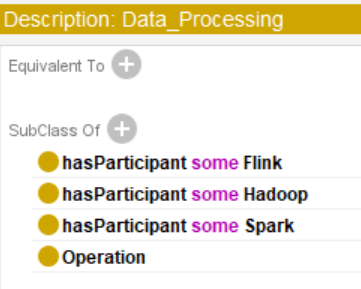
\includegraphics{docs/images/dataprocdesc.PNG}
    \caption{Descrizione di una sottoclasse di Operation: in questo caso Data Processing e le sue relazioni.}
    \label{fig:dataprocdesc}
\end{figure}

Nel contesto dei Big Data, un dominio estramemente frizzante in cui vengono definiti nuovi concetti giorno dopo giorno, è estramemnte probabile che estensioni e approfondimenti delle operazioni qui definite vengano aggiunte. In tale caso, la classe Operation si presta bene a nuove estensioni o migliorie.


\section{Server}
L'hardware rappresenta la "parte tangibile" di un sistema informatico o di un dispositivo elettronico. Un hardware può essere chiaramente anche il sistema informatico stesso come un telefono o un laptop. Le componenti hardware di tali sistemi sono gli stessi presenti in un computer, nodo o server, più in generale, che ci permettono di elaborare grandi quantità di dati. Da questa analisi è nata la classe \textbf{Server}, una classe che estende l'ontologia Hardware Ontology \cite{Hardware_Ontology} e che rappresenta appunto un una  macchina in grado di elaborare, gestire ed archiviare grandi volumi di dati. Di base, questi calcolatori sono usati in combinazione con loro simili. Inoltre, le specifiche tecniche di questi server sono paragonabili a computer di fascia alta.

\begin{figure}[H]
    \centering
    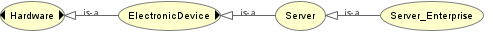
\includegraphics[width=12cm]{docs/images/bdhwowlviz.png}
    \caption{Gerarchia dalla classe Hardware creata su Protègè tramite il plugin OWLViz.}
    \label{fig:bdhw_graph}
\end{figure}

Le compomenti fisiche come la CPU, la RAM eccetera eccetera, danno vita ai server. Volendo modellare quest'ultimo concetto, ci siamo trovati dinanzi alla necessità di dover progettare a cascata tutti i concetti che compongono questi server (come detto, CPU, RAM, ecc.). L'impiego dell'ontologia Hardware Ontology \cite{Hardware_Ontology} è stato di estrema importanza: ci ha permesso di riutilizzare classi già da essa definite.\\
 
I server che tipicamente si impiegano sui progetti di Data Science o Big Data si definiscono in Server Commodity, ovvero dei server meno performanti e affidabili; per brevità questa classe è stata decisa di chiamarla più semplicemente \textbf{Server}. Quei server più affidabili e con prestazioni migliori vengono definiti \textbf{Server Enterprise}. Inizialmente volevamo rendere una Defined Class anche questa classe. Il solo OWL però non permetteva la modellazione ciò che avremmo voluto fare:  vedremo nel successivo capitolo, in particolare in \ref{sec:swrl}, come il reasoner ed in particolare le regole \textbf{SWRL} ci hanno aiutato in questo compito.
\chapter{Interrogazione dell'ontologia}
Questo capitolo esplora dettagliatamente le regole SWRL e le query SPARQL sviluppate durante il progetto, illustrando come queste tecniche siano state implementate per arricchire la fruibilità dell'ontologia.\\

Le regole SWRL forniscono un meccanismo potente per inferire nuove conoscenze all'interno dell'ontologia, consentendo di dedurre informazioni aggiuntive sulla base delle relazioni e delle proprietà definite. Questo strumento si è rivelato fondamentale per estendere la completezza dell'ontologia e fornire una visione più approfondita del dominio. Mentre, le query SPARQL rappresentano uno strumento essenziale per recuperare informazioni specifiche dall'ontologia. Attraverso l'utilizzo di SPARQL, è possibile eseguire interrogazioni complesse che permettono di individuare istanze specifiche dall'ontologia.

\section{SWRL}\label{sec:swrl}
All'interno di questa sezione, ci dedicheremo all'analisi delle regole SWRL, che sono state integrate nell'ontologia BDOnto. Queste regole sono state concepite con l'obiettivo di inferire nuove informazioni o di assegnare classificazioni alle istanze presenti nell'ontologia in base a specifiche condizioni. Ciascuna di queste regole svolge un ruolo distintivo all'interno del complesso processo di arricchimento dell'ontologia.\\

In totale sono state create 5 regole SWRL, che permettono di calcolare:
\begin{itemize}
    \item \texttt{BDOnto - Server Definition}: identifica quali istanze di Desktop possono essere anche Server in base ad alcune caratteristiche: il computer deve avere almeno una CPU con frequenza di Clock di 3 GHz, 8 GB di RAM e 500 GB di disco fisico.
    \item \texttt{BDOnto - Server Enterprise Definition}: identifica quali istanze di Desktop possono essere anche Server Enterprise in base ad alcune caratteristiche: il computer deve avere almeno una CPU con frequenza di Clock di 3 GHz, 8 GB di RAM, 500 GB di disco fisico e una GPU con 2 GB di memoria dedicata.
    \item \texttt{BDOnto - hasPlatform Definition}: stabilisce quale è la piattaforma/compagnia che si occupa di una data tecnologia sulla base del suo nome completo.
    \item \texttt{BDOnto - hasVersion Definition}: stablisce quale sia la versione di una tecnologia sulla base del nome completo.
    \item \texttt{BDOnto - hasLifespan Definition}: si calcola per quanti mesi una tecnologia è stata supportata.
\end{itemize}

\subsection{Premessa}\label{subsec:premswrl}
Data la natura del linguaggio SWRL alcune regole che avremmo voluto sviluppare non sono state possibili. Ad esempio, avremmo voluto creare una interrogazione che comprendesse una negazione. La negazione, a causa del principio di monotonicità che implica che una volta che si acquisiscono nuove informazioni, queste non vengono negate o rimosse, non è ammessa in SWRL.\\

Inoltre, volevamo utilizzare SWRL per estrapolare informazioni di diversa natura (es. la durata totale del supporto ad una tecnologia) e, tramite questo percorso, approfondire le nostre conoscenze a riguardo. In un primo momento è stata effettuata un'analisi di come avremmo potuto implementare queste regole. Dalle prime ricerche abbiamo individuato le Built-Ins per le date, definite dal W3C \cite{datetime_builtin} e la SWRL Temporal Built-In Library \cite{SWRLTemporalBuiltInsBasic}. I problemi con la prima soluzione sono nati in fase di reasoning. Infatti il reasoner utilizzato da noi, e maggiormente consigliato Pellet \cite{pelletreasoner}, supporta solo le prime 5 built-ins temporali del W3C \cite{datetime_builtin} (si veda \cite{pelletsupporttime}): ne risultava una scarsa "potenza" di approfondimento delle informazioni. Siamo poi passati all'impiego della libreria \texttt{temporal} \cite{SWRLTemporalBuiltInsBasic}. Dopo tanti tentativi, siamo riusciti ad utilizzarla a dovere e a costruire una regola che impiegasse tale costrutto \ref{subsec:haslifespan}.\\

Alcune piccole note tecniche. Nel caso in cui, anche dopo aver fatto partire il reasoner, alcune data properties che dovrebbero essere inferite non vengono mostrate a schermo, probabilmente non avete spuntato la casella per la visualizzazione di tali proprietà. Poi, nell'interfaccia principale di Protègè, bisogna andare in \texttt{Reasoner -> Configure -> Displayed inferences} e spuntare tutte le caselle relative alle data properties. Inoltre, il reasoner Pellet non supporta la libreria \texttt{temporal} \cite{SWRLTemporalBuiltInsBasic}, quindi per ottenere le informazioni relative al lifespan contenute in \ref{subsec:haslifespan} si deve:
\begin{itemize}
    \item Aprire una tab per il plugin SWRLTab;
    \item Cliccare il bottone \texttt{OWL+SWRL->Drools} e aspettare che termini;
    \item Cliccare il bottone \texttt{Run Drools} e aspettare che termini;
    \item A questo punto le informazioni sono state inferite ma ancora non vengono mostrate. Per mostrarle a schermo dobbiamo cliccare \texttt{Drools->OWL}. Facendo ciò molte informazioni verranno nuovamente aggiunte alla ontologia in maniera permanente. Se si vuole lasciare l'ontologia "pulita" è importante \textbf{non} salvare dopo aver fatto questo ultimo passaggio. Per ulteriori informazioni si faccia riferimento alla documentazione ufficiale del plugin \cite{SWRLTabplugin}.
\end{itemize}
Può capitare che la prima volta che si apre il file dell'ontologia all'interno di Protègè, e si ripete il processo definitio qui sopra per inferire le regole SWRL, vengano restituiti degli errori. Se per esempio viene rilevato un errore sulla regola \texttt{hasVersion}, copiare e incollare la regola definita in questo documento all'interno della regola definita in Protègè, salvare il file e poi ricaricare Protègè (\texttt{File -> Reload}). A questo punto l'errore dovrebbe scomparire.\\

Infine, nelle regole SWRL che mostriamo viene spesso ripetuta il predicato \texttt{swrlb:stringConcat}. Tale predicato è una sorta di soluzione alternativa al type conversion. Infatti, durante la realizzazione di queste regole SWRL, che dovevano funzionare in maniera uguale sia sul reasoner Pellet che sul reasoner del plugin SWRLTab, si sono affrontati spesso degli errori di conversione (es. \textit{cannot convert value of type PlainLiteral to xsd:string}). Il costo per la buona riuscita di tali regole in entrambi gli ambienti è stato l'incremento di complessità dato dall'aggiunta di tale predicato.\\

I tool impiegati in questa fase sono stati \textbf{Protègè} \cite{protegehomepage} ed il suo plugin \textbf{SWRLTab} \cite{SWRLTabplugin}.
\newpage 
\subsection{Server}
Questa regola è stata definita per meglio classificare quelle istanze di un computer che equivalgono ad una istanza di un server. Chiaramente alcune proprietà devono essere soddisfatte come la potenza della CPU (almeno 3 GHz di frequenza), la capacità della RAM (almeno 8 GB) e la disponibilità di memoria (almeno 500 GB). Di seguito la regola SWRL creata.\\

\begin{lstlisting}[language=Prolog]
Desktop(?d) ^
   cpuSpeedUnit(?d, ?us) ^ 
   cpuSpeedValue(?d, ?vs) ^
   deviceRAMUnit(?d, ?uc) ^
   deviceRAMValue(?d, ?vc) ^
   deviceStorageUnit(?d, ?ud) ^
   deviceStorageValue(?d, ?vd) ^
   swrlb:stringConcat(?sus, ""^^rdf:PlainLiteral, ?us)
   swrlb:stringEqualIgnoreCase(?sus, "GHz") ^
   swrlb:greaterThanOrEqual(?vs, 3.0) ^
   swrlb:stringConcat(?suc, ""^^rdf:PlainLiteral, ?uc)
   swrlb:stringEqualIgnoreCase(?suc, "GB") ^
   swrlb:greaterThanOrEqual(?vc, 8) ^
   swrlb:stringConcat(?sud, ""^^rdf:PlainLiteral, ?ud)
   swrlb:stringEqualIgnoreCase(?sud, "GB") ^
   swrlb:greaterThanOrEqual(?vd, 500) ->
   Server(?d)
\end{lstlisting}
\newpage
\subsection{Server Enterprise}
Questa regola, che risulta essere una estensione della precedente, definisce come classificare quei Desktop che hanno caratteristiche comuni ad i server enterprise. Le proprietà che devono rispettare sono le stesse dei server classici, con l'aggiunta di una GPU con almeno 2 GB di memoria dedicata. Di seguito la regola SWRL creata.\\

\begin{lstlisting}[language=Prolog]
Desktop(?d) ^
   hasGPU(?d, ?gpu) ^
   gpuMemoryUnit(?d, ?ug) ^
   gpuMemorySize(?d, ?vg) ^		
   cpuSpeedUnit(?d, ?us) ^ 
   cpuSpeedValue(?d, ?vs) ^
   deviceRAMUnit(?d, ?uc) ^
   deviceRAMValue(?d, ?vc) ^
   deviceStorageUnit(?d, ?ud) ^
   deviceStorageValue(?d, ?vd) ^
   swrlb:stringConcat(?sus, ""^^rdf:PlainLiteral, ?us)
   swrlb:stringEqualIgnoreCase(?sus, "GHz") ^
   swrlb:greaterThanOrEqual(?vs, 3.0) ^
   swrlb:stringConcat(?suc, ""^^rdf:PlainLiteral, ?uc)
   swrlb:stringEqualIgnoreCase(?suc, "GB") ^
   swrlb:greaterThanOrEqual(?vc, 8) ^
   swrlb:stringConcat(?sud, ""^^rdf:PlainLiteral, ?ud)
   swrlb:stringEqualIgnoreCase(?sud, "GB") ^
   swrlb:greaterThanOrEqual(?vd, 500) ^
   swrlb:stringConcat(?sug, ""^^rdf:PlainLiteral, ?ug)
   swrlb:stringEqualIgnoreCase(?sug, "GB") ^
   swrlb:greaterThanOrEqual(?vg, 2) ->
   Server_Enterprise(?d)
\end{lstlisting}
\newpage
\subsection{hasPlatform}
Questa regola serve ad associare una azienda ad una tecnologia. La motivazione di tale regola risiede nel fatto che può essere ripetitivo scrivere a quale compagnia è associato un certo prodotto. L'obiettivo è quindi quello di estrapolare dalle proprietà già definite all'interno di una istanza di \textit{Big\_Data\_Technology} questa informazione. E lo fa prima, estraendo il nome completo della tecnologia e di una azienda (\textit{Company}), successivamente, confronta se il nome completo della tecnologia contiene il nome completo della compagnia (ignorando le differenze tra maiuscole e minuscole) ed infine, se questa condizione è soddisfatta, la regola crea un collegamento tra le due istanze assegnando loro la proprietà \textbf{hasPlatform}. Di seguito la regola SWRL creata.\\

\begin{lstlisting}[language=Prolog]
Big_Data_Technology(?d) ^ 
   hasFullName(?d, ?dname) ^ 
   Company(?c) ^
   companyName(?c, ?cname) ^
   swrlb:stringConcat(?ddname, ""^^xsd:string, ?dname) ^
   swrlb:stringConcat(?dcname, ""^^xsd:string, ?cname) ^
   swrlb:containsIgnoreCase(?ddname, ?dcname) -> hasPlatform(?d, ?c)
\end{lstlisting}

\subsection{hasVersion}
Questa regola, è stata progettata per estrarre informazioni sulla versione di una data tecnologia partendo dal nome completo di essa. Come nei casi precedenti, anche qui sfruttiamo un predicato built-in di SWRL chiamato \textit{substringAfter} che ritorna tutto ciò che è dopo un determinato carattere data una stringa in ingresso. In generale quindi, si parte dal nome completo, si separa la parte dove si specifica la versione (è stato deciso che per inferire questa informazione deve essere presente nel nome completo la "V" che farà da divisore) e quest'ultima verrà inserita nella data property \textit{hasVersion}. Di seguito la regola SWRL creata.\\

\begin{lstlisting}[language=Prolog]
Big_Data_Technology(?d) ^ 
   hasFullName(?d, ?name) ^
   swrlb:stringConcat(?dname, ""^^xsd:string, ?name)
   swrlb:substringAfter(?version, ?dname, "V"^^xsd:string) -> hasVersion(?d, ?version)
\end{lstlisting}
\newpage
\subsection{hasLifespan} \label{subsec:haslifespan}
Questa regola SWRL è stata progettata per calcolare la durata di vita di una tecnologia Big Data. Per durata di vita intendiamo il tempo nel quale tale tecnologia è stata supportata ufficialmente. Si parte dalla data di introduzione sul mercato della tecnologia e dalla data di fine supporto. In seguito il predicato \texttt{duration} calcolerà per quanti mesi è stata supportato tale prodotto. Di seguito la regola SWRL creata.\\

\begin{lstlisting}[language=Prolog]
Big_Data_Technology(?d) ^ 
   hasStartingDate(?d, ?startTime) ^ 
   hasEndOfSupportDate(?d, ?endTime) ^ 
   swrlb:stringConcat(?dstartTime, ""^^rdf:PlainLiteral, ?startTime) ^
   swrlb:stringConcat(?dendTime, ""^^rdf:PlainLiteral, ?endTime)
   temporal:duration(?lifeSpan, ?dstartTime, ?dendTime, "Months"^^xsd:string) -> hasLifespan(?d, ?lifeSpan)
\end{lstlisting}
\newpage

\section{SPARQL}\label{sec:sparql}
In questa sezione, esamineremo le query SPARQL implementate in BDOnto, le quali sono state sviluppate per estrarre informazioni significative attraverso criteri specifici.\\

Le query da noi sviluppate sono:
\begin{itemize}
    \item \textit{Quali sono i tre linguaggi di programmazione più supportati}: si calcolano i tre linguaggi di programmazione più utilizzati dai vari tool. Una query di questo tipo potrebbe risultare importante, ad esempio per un neofita del mondo Big Data, per capire da quale linguaggio partire nel suo percorso di studi.
    \item \textit{Quali tecnologie non sono più supportate}: si valutano quali tecnologie non hanno più un supporto dalla casa produttrice. Una query di questo genere potrebbe aiutare nella scelta della versione di un tool da utilizzare, ad esempio.
    \item \textit{Numero di istanze di Big Data Tool usati negli step di Data Visualization}: si trova il numero di volte che un dato tool è stato impiegato negli step di Data Visualization. Una query del genere potrebbe tornare utile nel momento in cui si vuole effettuare una analisi quantitativa sulla distribuzione dell'uso degli strumenti all'interno dei processi di visualizzazione dei dati.
    \item \textit{Quali sono le tre tecnologie con il tempo di supporto più lungo}: si analizzano quali tecnologie hanno avuto supporto per più a lungo, limitando il risultato alle tre tecnologie con durata maggiore. Questa query potrebbe essere molto utile durante una fase iniziale di un progetto: ordinando le tecnologie in base alla durata della vita più lunga, è possibile identificare quelle che hanno una maggiore stabilità nel tempo o che hanno una prospettiva di supporto a lungo termine.
    \item \textit{Quali tecnologie hanno raggiunto almeno la terza versione e tale versione è supportata}: si valutano le tecnologie che hanno raggiunto un certo grado di maturità (assumiamo che sia almeno la terza versione) e che tale versione sia ancora supportata dal team di sviluppo. Tale query potrebbe essere interessante per chi deve decidere quale versione di un software scegliere, se aggiornare o meno una versione già impiegata o per una semplice analisi sul supporto di una data tecnologia; in generale può avere tanti propositi.\\
    
    \item \textit{Quali Server sono supportati da AWS e hanno almeno 16GB di RAM ed una GPU}: questa query identifica i server adatti per essere utilizzati da un servizio come AWS, specificando i requisiti come una capacità di almeno 16 GB di RAM e la presenza di una GPU. Tale interrogazione potrebbe risultare utile per coloro che intendono scegliere un servizio e conoscono i requisiti tecnici necessari; una query simile potrebbe elencare tutte le soluzioni infrastrutturali disponibili.
\end{itemize}


\subsection{Premessa}
Per evitare di ripetere diverse volte i prefissi utilizzati nelle query, li riportiamo solamente in questa sezione.

\begin{figure}[H]
    \centering
    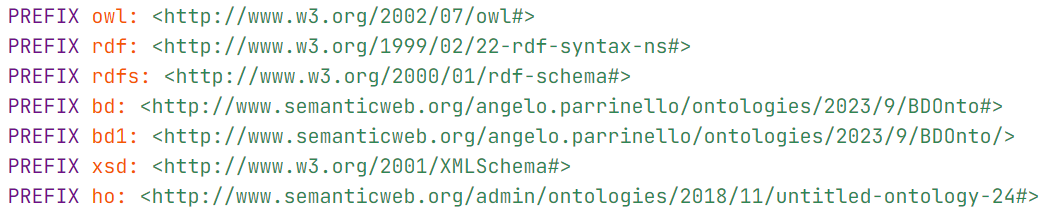
\includegraphics[width=15cm]{docs/images/prefix.PNG}
    \caption{Prefissi usati nelle query SPARQL.}
    \label{fig:prefix}
\end{figure}
In questa fase risulta di vitale importanza attivare il reasoner prima di lanciare qualunque query SPARQL all'interno di Protègè. Infatti il plugin per le query SPARQL di Protègè ha alcuni problemi tra cui alcuni legati all'UI: infatti se il reasoner è selezionato ma non attivo, alla richiesta di una query questo tornerà un risultato vuoto (si veda \cite{sparqluibug}).\\

Queste query sono state create usando \textbf{Protègè}, il suo plugin \textbf{Snap SPARQL Query} \cite{snapsparqlquery} e \textbf{GraphDB} \cite{graphdbhomepage}. In particolare, le query 2 e 6 sono state sviluppate e testate tramite GraphDB a causa di alcuni problemi legati a Protègè.
\newpage
\subsection{Query 1 - Tre Linugaggi più Popolari}
Questa query SPARQL consente di identificare i tre linguaggi di programmazione più supportati dal pool di strumenti big data presenti in questa ontologia. Le variabili \texttt{?language} e \texttt{?supportCount} vengono utilizzate per selezionare e contare, rispettivamente. Nella clausola \texttt{WHERE}, si devono rispettare certe condizioni: le variabili devono essere del tipo corretto e deve esistere una relazione tra di loro. La clausola \texttt{GROUP BY} raggruppa i risultati in base a \texttt{?language} che poi vengono ordinati in modo decrescente in base al numero di strumenti che supportano ciascun linguaggio. Infine, \texttt{LIMIT 3} limita i risultati alle prime tre occorrenze. Di seguito la query SPARQL prodotta.\\

\begin{lstlisting}[language=SQL]
SELECT ?language (COUNT(?tool) AS ?supportCount)
WHERE {
  ?language rdf:type bd:Programming_Language.
  ?tool rdf:type bd:Big_Data_Tool.  
  ?language bd:supportedBy ?tool.
}
GROUP BY ?language
ORDER BY DESC(?supportCount)
LIMIT 3
\end{lstlisting}


\subsection{Query 2 - Tecnologie non più supportate}
La seguente query SPARQL seleziona le tecnologie per i Big Data senza più supporto confrontando la data di fine del supporto di ciascuno strumento con la data attuale. Recupera le variabili \texttt{?tool, ?endDate} e \texttt{?currentDate}, filtra le istanze della classe corretta, recupera la data di fine supporto, ricava l'istante attuale con la funzione \texttt{NOW()} (che ritorna un tipo \texttt{xsd:dateTime} quindi direttamente confrontabile con le nostre date tramite l'operatore \texttt{<}) ed infine filtra solo gli strumenti la cui data di fine del supporto è precedente alla data attuale. I risultati sono ordinati in base alla data di fine del supporto in ordine ascendente. Di seguito la query finale.\\
\newpage
\begin{lstlisting}[language=SQL]
SELECT ?tool ?endDate ?currentDate
WHERE {
  ?tool rdf:type bd:Big_Data_Technology.
  ?tool bd:hasEndOfSupportDate ?endDate.
  BIND(NOW() AS ?currentDate)
  FILTER (?endDate < ?currentDate)
}
ORDER BY ASC(?endDate)
\end{lstlisting}
\subsection{Query 3 - Numero di Tool impiegati negli step di 'Data Visualization'}
L'intenzione di questa query SPARQL è estrarre informazioni sul numero di tool usati in ogni step di tipo \textit{Data\_Visualization}, tramite le operazione ad esso associate. Sapendo che ogni istanza di \textit{Data\_Visualization} è associata ad una operazione e che quest'ultima è associata a sua volta ad un tool, arriviamo a contare il numero univoco di istanze di \textit{Big\_Data\_Tool} collegate. Di seguito la query SPARQL creata.\\

\begin{lstlisting}[language=SQL]
SELECT ?tool (COUNT(DISTINCT ?dataVisualization) AS ?toolCount)
WHERE {
  ?dataVisualization rdf:type bd:Data_Visualization.
  ?dataVisualization bd:consistsOf ?operation.
  ?operation rdf:type bd:Operation.
  ?operation bd:hasParticipant ?tool.
}
GROUP BY ?tool
ORDER BY DESC(?toolCount)
\end{lstlisting}
\newpage
\subsection{Query 4 - Tre Tool con il tempo di supporto più lungo}
Prima di lanciare questa query è importante inferire l'informazione contenuta in \texttt{hasLifespan} (seguendo il percorso definito in \ref{subsec:premswrl}). La query filtra le istanze di tipo \texttt{Big\_Data\_Technology} e ne recupera il valore di \texttt{hasLifespan}. Infine, recupera le 3 tecnologie big data con il tempo di supporto più lungo, ordinando le istanze in modo decrescente sulla base dei tempi.\\

\begin{lstlisting}[language=SQL]
SELECT ?technology ?lifespan
WHERE {
  ?technology rdf:type bd:Big_Data_Technology.
  ?technology bd:hasLifespan ?lifespan.
}
ORDER BY DESC(?lifespan)
LIMIT 3
\end{lstlisting}

\subsection{Query 5 - Tecnologie con almeno la versione 3 e che sono tutt'ora supportate}
La seguente query SPARQL elenca le tecnologie che sono arrivati ad almeno la terza versione e che tale versione è supportata. Dopo aver selezionato le tecnologie, la propria versione ed eventualmente il nome completo (notare la clausola \texttt{OPTIONAL} che permette di includere le tecnologie che potrebbero non avere un nome completo, quindi non è una condizione vincolante), si cerca di recuperare anche la data di fine del supporto. Anche il recupero di tale campo risulta essere opzionale. L'operatore \texttt{bound} consente di verificare se una variabile è stata assegnata ad un valore. In questo specifico caso controlliamo se \texttt{endDate} è collegata alla tecnologia in questione o in altre parole controlliamo se l'istanza presa in considerazione ha associata una proprietà del tipo \texttt{hasEndOfSupportDate}. Quindi nella seconda \texttt{FILTER} filtriamo quelle tecnologie che o non hanno una data di fine supporto (e quindi assumiamo che siano ancora supportate) oppure tale data è antecedente al momento corrente. La seconda clausola di filtering  è importante che sia opzionale. Infatti, tale blocco rende la condizione sulla data di fine del supporto non vincolante per l'inclusione di una tecnologia nella risultante e quindi, se una tecnologia non ha una data di fine del supporto, viene comunque inclusa nella risultante. Infine, le istanze rimanenti vengono nuovamente filtrare in base al numero di versione. Di seguito la query creata.
\newpage
\begin{lstlisting}[language=SQL]
SELECT ?technology ?version ?fullName ?endDate
WHERE {
  ?technology rdf:type bd:Big_Data_Technology.
  ?technology bd:hasVersion ?version.
  OPTIONAL {?technology bd:hasFullName ?fullName.}
  OPTIONAL {
    ?technology bd:hasEndOfSupportDate ?endDate.
    BIND(NOW() AS ?currentDate)
    FILTER (!bound(?endDate) || ?endDate > ?currentDate)
  }
  FILTER (?version >= "3.0.0")
}
\end{lstlisting}

\subsection{Query 6 - Server supportati da AWS con almeno 16GB di RAM ed una GPU}
La seguente query evidenzia gli individui della classe Server, supportati dal servizio AWS e con almeno 16GB di RAM ed una GPU. Di seguito la query svluppata. Da notare la clausola \texttt{OPTIONAL} che controllo che almeno una proprietà legata alla GPU sia presente per definire o meno la presenza della stessa.
\begin{lstlisting}[language=SQL]
SELECT ?server
WHERE {
    ?server rdf:type bd1:Server.
    ?awsService rdf:type bd1:AWS.
    ?awsService bd:supportsWith ?server.
    
    ?server ho:deviceRAMUnit "GB"^^xsd:string.
    ?server ho:deviceRAMValue ?ramValue.
    FILTER(?ramValue >= 16)
    
    OPTIONAL {
        ?server ho:gpuMemoryUnit ?gpuMemoryUnit.
        ?server ho:gpuMemorySize ?gpuMemorySize.
        ?server ho:hasGPU ?hasGPU.
        FILTER (bound(?gpuMemoryUnit) || bound(?gpuMemorySize) || bound(?hasGPU) )
    }
}
\end{lstlisting}
\chapter{Valutazioni Finali}

\section{Conclusioni}
La creazione di questa ontologia dedicata alle tecnologie Big Data e al processo di Data Science pensiamo possa essere uno strumento di supporto al processo decisionale efficace. L'ontologia fornisce un insieme ben strutturato di classi, proprietà e regole SWRL che consentono di estrarre informazioni rilevanti sulle tecnologie, i software e le operazioni nel dominio del Big Data.\\

Nonostante sia ancora incompleta, la sua progettazione offre una base robusta per future espansioni e sviluppi. L'obiettivo iniziale di incorporare un ampio spettro di informazioni in modo logico per rendere l'ontologia accessibile anche agli utenti esterni è stato raggiunto. Va sottolineato che, essendo un progetto universitario, l'attenzione principale è stata rivolta alla comprensione approfondita del Web Semantico, esplorando diverse componenti di ciascun aspetto, come le regole SWRL e le query SPARQL. In aggiunta, nel corso dell'approfondimento, abbiamo dovuto confrontarci con le limitazioni degli strumenti utilizzati, spingendoci a ricorrere a nuove tecniche o tecnologie. Questa sfida ci ha motivato ad ampliare ulteriormente le nostre conoscenze. Nel complesso, siamo soddisfatti del risultato ottenuto e riteniamo di aver raggiunto l'obiettivo prefissato.

\section{Sviluppi futuri}
Per migliorare ulteriormente l'efficacia dell'ontologia, sarebbe benefico ampliare il dominio con una gamma più ampia di tecnologie e linguaggi di programmazione, nonché incorporare gli ultimi sviluppi legati alla Data Science. Questo arricchimento consentirebbe di ottenere una panoramica più dettagliata delle tecnologie utilizzate nel contesto dei Big Data e agevolerebbe il processo di sviluppo di progetti di Data Science. Introducendo nuove definizioni di classi, insieme alla creazione di proprietà e regole supplementari, si potrebbe modellare scenari più complessi e specifici, migliorando la precisione delle inferenze effettuate dal reasoner.

\bibliographystyle{plain}
\bibliography{bibliography}

\end{document}